\documentclass{report}
\usepackage[utf8]{inputenc}
\usepackage{natbib}
\usepackage{graphicx}
\usepackage[italian]{cleveref}
\usepackage[italian]{babel}
\usepackage{subfigure}
\usepackage{wrapfig}
\usepackage{dirtree}
\usepackage{xcolor}
\usepackage[section]{placeins} % figures before next section
\usepackage{listings}

\usepackage{color}
\definecolor{lightgray}{rgb}{.9,.9,.9}
\definecolor{darkgray}{rgb}{.4,.4,.4}
\definecolor{purple}{rgb}{0.65, 0.12, 0.82}

\lstdefinelanguage{JavaScript}{
  keywords={typeof, new, true, false, catch, function, return, null, catch, switch, var, if, in, while, do, else, case, break},
  keywordstyle=\color{blue}\bfseries,
  ndkeywords={class, export, boolean, throw, implements, import, this},
  ndkeywordstyle=\color{darkgray}\bfseries,
  identifierstyle=\color{black},
  sensitive=false,
  comment=[l]{//},
  morecomment=[s]{/*}{*/},
  commentstyle=\color{purple}\ttfamily,
  stringstyle=\color{red}\ttfamily,
  morestring=[b]',
  morestring=[b]"
}

\lstset{
   language=JavaScript,
   backgroundcolor=\color{lightgray},
   extendedchars=true,
   basicstyle=\footnotesize\ttfamily,
   showstringspaces=false,
   showspaces=false,
   numbers=left,
   numberstyle=\footnotesize,
   numbersep=9pt,
   tabsize=2,
   breaklines=true,
   showtabs=false,
   captionpos=b
}

\definecolor{codegray}{gray}{0.925}
\newcommand{\code}[1]{\colorbox{codegray}{\texttt{\detokenize{#1}}}}
\newenvironment{codeblock}[1]{\colorbox{codegray}{\texttt{\detokenize{#1}}}}

\title{
    MyWaste \\
    \large Applicazioni e Servizi Web
}

\author{Federico Pettinari - 988120 \{federico.pettinari2@studio.unibo.it\}\\
Hamado Dene - 973128 \{hamado.dene@studio.unibo.it\}}
\date{\today}

\begin{document}

\maketitle
\section{Introduzione}
%Introduzione \citep{adams1995hitchhiker}
Lo scopo del progetto è la realizzazione di un'applicazione web per la gestione dei dati dei rifiuti cittadini ed i relativi conferimenti,
in modo che ogni cittadino possa sapere (anche in tempo reale) la quantità ed il costo dei rifiuti prodotti.
A questo scopo si presume che ogni cassonetto per la raccolta differenziata sia dotato di lettore RFID per poterne identificare
il padrone in modo automatico.

\section{Requisiti}
\begin{itemize}
    \item Progettare e sviluppare una web app per la visualizzazione e gestione dei dati sui rifiuti cittadini
    \item I cassonetti sono dotati di sensore di peso e lettore rfid per identificare l’utente che sta conferendo i rifiuti
    \item La piattaforma deve calcolare il costo mensile in funzione del tipo di rifiuto e peso.
    \item Deve mostrare la notifica del conferimento all’utente
    \item Deve mostrare grafici statistici sul conferimento
    \item La lettura dei sensori dei cassonetti ed il conseguente inserimento dei dati sull'applicazione
    avvengono automaticamente al centro di smistamento, senza bisogno di intervento da parte dell'utente.
\end{itemize}

\section{Design}
\subsection{Architettura}
L'architettura è raffigurata in \Cref{fig:arch}.
Ogni richiesta HTTP viene ricevuta e smistata dal reverse proxy.
Le chiamate che iniziano con /api vengono passate al backend, mentre le altre al frontend.
Questo aiuta a separare frontend e backend in modo trasparente e senza bisogno di utilizzare Cross-Origin Resource Sharing (CORS).

\begin{figure}[h!]
\centering
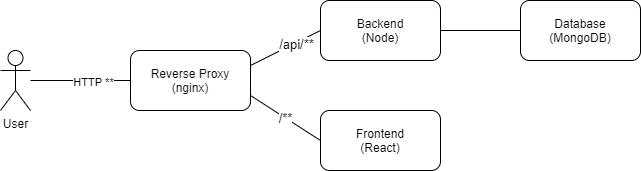
\includegraphics[width=\textwidth]{arch}
\caption{Architettura}
\label{fig:arch}
\end{figure}

\subsection{Database}
Il modello del database è semplice e raffigurato in \Cref{fig:db}. L'applicazione può avere un numero variabile di account.
Ad ogni account sono associate le proprie notifiche e conferimenti (Waste). Un account oltre ai dati di identificazione
(email e password), ha un ruolo (role) per distinguere amministratori da utenti. Per ogni conferimento vengono memorizzati
la data, il tipo di spazzatura (es. plastica o carta) e la quantità. Per ogni notifica vengono memorizzati la data di creazione,
una flag per sapere se è stata letta, ed il tipo e quantità per i conferimenti.
\begin{figure}[h!]
    \centering
    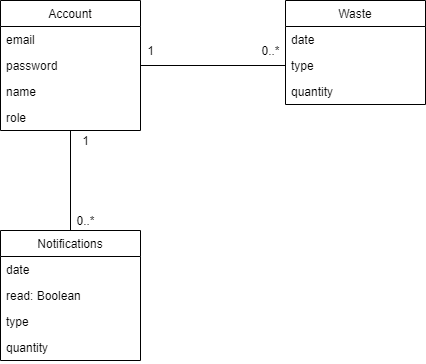
\includegraphics[width=\textwidth]{db}
    \caption{Modello del database}
    \label{fig:db}
\end{figure}

\subsection{Interfaccia utente}
Per il design dell'interfaccia utente è stato inizialmente sviluppato il mockup raffigurato in \Cref{fig:mockup}, che si è
man mano evoluto a seguito dei test di usabilità effettuati. E' stata prediletta la semplicità e l'immediatezza.
Il progetto nasce mobile-first con interfaccia responsive per supportare anche schermi desktop.

\begin{figure}[h!]
    \centering
    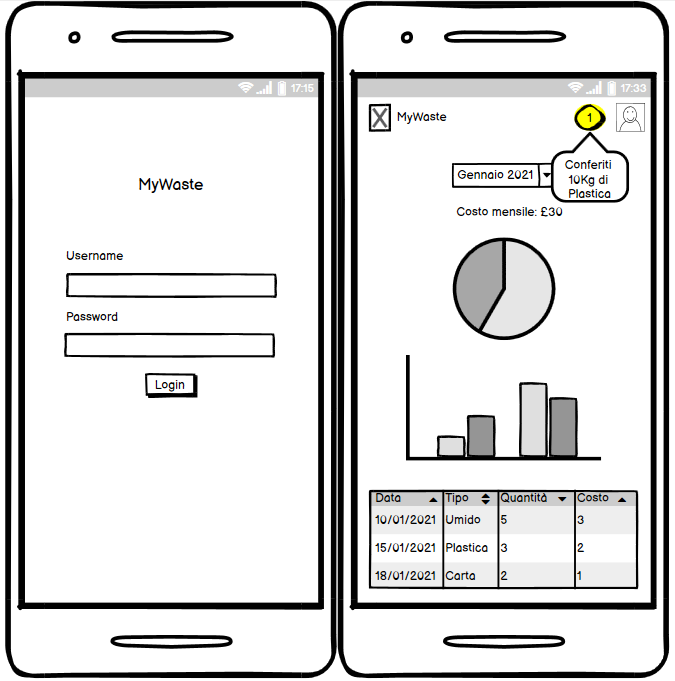
\includegraphics[width=\textwidth]{mockup}
    \caption{Mockup interfaccia utente}
    \label{fig:mockup}
\end{figure}

\section{Tecnologie}
Il progetto utilizza le seguenti tecnologie:
\begin{itemize}
    \item Github Actions - per continous integration
    \item Docker - per disaccoppiare il software dal sistema operativo e facilitarne il porting ed installazione.
    \item nginx - utilizzato come reverse proxy
    \item MongoDB - database non relazionale di documenti
    \item Node - come server web sia per frontend e backend
    \item Express - framework per gestire chiamate e routes HTTP
    \item Mongoose - come libreria di object modeling per mongodb
    \item Mocha e Supertest - per testing automatizzato nel backend
    \item mongodb-memory-server - per utilizzare un database mongodb in memoria, in modo da velocizzare l'esecuzione dei test
    \item bcrypt - per criptare le password degli utenti ai fini di sicurezza
    \item express-jwt - libreria per facilitare l'uso di tokens JWT utilizzati nel sistema di login utente
    \item Nodemon - tool che riavvia le applicazioni Node ad ogni modifica del sorgente
    per velocizzarne lo sviluppo e debugging
    \item React - framework per frontend
    \item SCSS - estensione di CSS che ne facilita il riuso
    \item Bootstrap - framework per CSS
\end{itemize}

\section{Codice}
\subsection{Backend}
Il backend è costituito da un servizio che espone API RESTful in formato JSON, ed è sviluppato con le tecnologie principali
Node, Express e database MongoDB.
\subsubsection{APIs}
Le API implementate sono:
\begin{itemize}
    \item \code{Post /login } Restituisce un json contente username,name,role e token JWT se i paramentri username e password passati
    nella fase di request risultano corretti.
    \item \code{Get /me } Restituisce le informazioni dell'utente loggato. La richiesta deve essere fatto usando un token valido.
    \item \code{Get /account } Restituisce la lista degli utenti registrati nella piattaforma. Questa api, può essere chiamata solo dagli utenti admin.
    \item \code{Post /account } Permette la creazione di nuovi account da parte di amministratori.
    \item \code{Patch /account/:account } Permette agli amminstratori di aggiornare le informazioni di un account esistente dato il suo id.
    \item \code{Delete /account/:account } Permette ad un amministratore di cancellare un account dalla piattaforma.
    \item \code{Post /waste } API per registrare i dati relativi ad un conferimento, come tipo e peso dei rifiuti.
    \item \code{Get /waste} Permette di effettuare query sui conferimenti, usando opportuni parametri quali:
        \begin{itemize}
            \item \code{groupByType} Per richiedere i dati aggregati per tipo di rifiuto.
            \item \code{includeDataPoints} Per includere la lista dei singoli dati in una query con raggruppamento.
            \item \code{from} Data di inizio
            \item \code{to} Data di fine
        \end{itemize}
    \item \code{Get /notifications } Restituisce la lista delle notifiche di un determinato account.
    \item \code{Patch /notifications/:notification } Permette di aggiornare lo stato della notifica a Read.
\end{itemize}

\subsubsection{Autenticazione}
Il backend gestisce l'autenticazione ed i permessi degli utenti.
Alla creazione di un account, la password viene criptata con algoritmo bcrypt e salvata su DB.
Quando viene richiesta l'autenticazione e i parametri (username e password) corrispondono ai parametri salvati su DB,
viene restituito un token JWT che permette l'accesso alla piattaforma. Esso contiene informazioni come id e permessi.
Di seguito parte del codice volto alla gestione di permessi ed autenticazione:
\begin{lstlisting}
const JWT_SECRET = '12345' // just for demonstration
const REQUEST_PROPERTY_DECODED_JWT = 'auth' // decoded JWT token gets inserted in request.auth

const jwt = require('jsonwebtoken')
// JWT decoding middleware
const auth = require('express-jwt')({ // JWT decoding middleware
    secret: JWT_SECRET,
    algorithms: ['HS256'],
    credentialsRequired: true,
    requestProperty: REQUEST_PROPERTY_DECODED_JWT
})
const guard = require('express-jwt-permissions')({
    requestProperty: REQUEST_PROPERTY_DECODED_JWT,
    permissionsProperty: 'role' // permissions are stored in the role field of the JWT token
})
//Generate token for user
module.exports = {
    auth: auth,
    guard: guard,
    createToken(account) {
        return jwt.sign({id: account._id, role:account.role}, JWT_SECRET)
    }
}
\end{lstlisting}

\begin{lstlisting}
//Account model
const mongoose = require('mongoose')
const bcrypt = require('bcrypt')
const { Schema } = mongoose

const accountSchema = new Schema({
    email: {
        type: String,
        unique: true,
        required: true
    },
    password: {
        type: String,
        required: true
    },
    role: {
        type: String,
        default: 'user'
    },
    name: {
        type: String,
        required: true
    }
})

accountSchema.pre('save', function(next) {
    if (!this.isModified('password')) {
        return next()
    }
    bcrypt.genSalt(2, (error, salt) => {
        if (error) {
            return next(error)
        }
        bcrypt.hash(this.password, salt, (error, hash) => {
            if (error) {
                return next(error)
            }
            this.password = hash
            next()
        })
    })
})

accountSchema.methods.toJSON = function() {
    var obj = this.toObject()
    delete obj.password
    obj.id = obj._id
    delete obj._id
    delete obj.__v
    return obj
}

module.exports = mongoose.model('Account', accountSchema)
\end{lstlisting}

\subsubsection{Rifiuti}
\begin{lstlisting}
//Waste model
const mongoose = require('mongoose')
const { Schema } = mongoose

const schema = new Schema({
    account: { type: Schema.Types.ObjectId, required: true, ref: 'Account' },
    type: { type: String, required: true },
    quantity: { type: Number, required: true },
    date: { type: Date, default: Date.now, required: true, index: true }
})
schema.index({account: 1, date: -1}) // ascending accounts, descending dates

module.exports = mongoose.model('Waste', schema, 'waste')
\end{lstlisting}

\begin{lstlisting}
//Waste controller
module.exports = {
    delivery(req, res, next) {
        Account.findById(req.body.account).exec()
            .then( acct => {
                let data = {
                    account: acct.id,
                    quantity: req.body.quantity,
                    type: req.body.type
                }
                if (req.body.date) {
                    data.date = new Date(req.body.date)
                }
                return new Waste(data).save()
            })
            .then(
                waste => {
                    new Notification({
                        account: waste.account,
                        date: waste.date,
                        message:`Delivered ${waste.quantity} Kg of ${waste.type}`
                    }).save()
                    res.status(201).json(waste)
                },
                err => next(err)
            )
    },
    query(req, res, next) {
        let q = null
        if (req.query.groupByType) {
            const pipeline = [
                {
                    $group: {
                        _id: "$type",
                        total: {$sum: "$quantity"}
                    }
                }, {
                    $project: {
                        _id: 0,
                        type: "$_id",
                        total: 1
                    }
                }
            ]
            if(req.query.includeDataPoints) {
                pipeline[0].$group.data = { $push:  { date: "$date", quantity: "$quantity" } }
                pipeline[1].$project.data = 1
            }
            let match = { }
            if (req.query.account) {
                match.account = ObjectId(req.query.account)
            }
            if (req.query.from) {
                match.date = { $gte: new Date(req.query.from) }
            }
            if (req.query.to) {
                match.date = match.date || {}
                match.date.$lte = new Date(req.query.to)
            }
            if(Object.keys(match).length > 0) {
                pipeline.unshift({ $match: match })
            }
            q = Waste.aggregate(pipeline)
        } else {
            q = Waste.find()
            if (req.query.account) {
                q.where('account', ObjectId(req.query.account))
            }
            if (req.query.from) {
                q.where('date').gte(new Date(req.query.from))
            }
            if (req.query.to) {
                q.where('date').lte(new Date(req.query.to))
            }
        }
        q.then(
            result => res.status(200).json(result),
            err => next(err)
        )
    }
}
\end{lstlisting}

\subsubsection{Notifiche}
Le notifiche vengono inserite automaticamente al momento del conferimento. Si presuppone che il frontend effettui polling.
\begin{lstlisting}
//Notification model
const mongoose = require('mongoose')
const { Schema } = mongoose

const notificationSchema = new Schema({
    read: {
        type: Boolean,
        default: false
    },
    date: {
        type: Date,
        default: Date.now
    },
    message: {
        type: String,
        required: true
    },
    account: { type: Schema.Types.ObjectId, required: true, ref: 'Account' },
})

module.exports = mongoose.model('Notification', notificationSchema)
\end{lstlisting}

\begin{lstlisting}
//Notifications controller
const Notification = require('../models/notification')

module.exports = {
    query(req, res, next) {
        let q = Notification.find({account: req.auth.id})
        if (req.query.from) {
            q.where('date').gte(new Date(req.query.from))
        }
        if (req.query.to) {
            q.where('date').lte(new Date(req.query.to))
        }
        q.sort({date:'descending'})
        q.exec().then(notifications => res.status(200).json(notifications), next)
    },
    markAsRead(req, res, next) {
        Notification.findByIdAndUpdate(req.params.notification, req.body, {new:true})
            .then(n => res.json(n), next)
    }
}
\end{lstlisting}

\subsection{Frontend}
Il frontend è costituito da un servizio web sviluppato con Node e React.
\subsubsection{Autenticazione}
L'autenticazione è delegata al backend attraverso l'apposita API di login.
Ricevuto il token JWT, esso viene salvato in localStorage per memorizzare la sessione.
\begin{lstlisting}
import React, { useState } from 'react';
import PropTypes from 'prop-types';

async function loginUser(credentials) {
    return fetch('/api/login', {
        method: 'POST',
        headers: {
            'Content-Type':'application/json'
        },
        body: JSON.stringify(credentials)
    }).then(
        data => data.json()
    )
}

export default function Login({setToken}) {

    const [email, setEmail] = useState();
    const [password, setPassword] = useState();
    const [errorMessage, setErrorMessage] = useState();

    const handleSubmit = async e => {
        e.preventDefault();
        const token = await loginUser({
            email,
            password
        });
        if(token) {
            setErrorMessage('Authentication error. Incorrect username or password.')
        }
        setToken(token);
    }
    return(...)
}


export default function useToken() {
  const getToken = () => {
    const tokenString = localStorage.getItem('token');
    const userToken = JSON.parse(tokenString);
    return userToken?.token
  };

  const [token, setToken] = useState(getToken());

  const saveToken = userToken => {
    localStorage.setItem('token', JSON.stringify(userToken));
    setToken(userToken.token);
  };

  return {
    setToken: saveToken,
    token
  }
}
\end{lstlisting}

\subsubsection{Gestione account}
\begin{lstlisting}
//Get users list
state = {
	users: []
}

getUserList() {
	fetch("/api/account", {
		method: 'GET',
		withCredentials: true,
		credentials: 'include',
		headers: {
			'Authorization': 'Bearer ' + JSON.parse(localStorage.getItem('token')).token ,
		}
	})
	.then(response => response.json())
	.then(json => {
		this.setState({users: json})
	}).catch((error) => {
	  alert("some error: " + error);
   });
}
\end{lstlisting}

\begin{lstlisting}
//Add user
handleAddUser() {
	if(this.state.user.length < 4) {
		alert("All fields are required!")
		return;
	}
	fetch("/api/account/", {
		method: 'POST',
		withCredentials: true,
		credentials: 'include',
		headers: {
			'Authorization': 'Bearer ' + JSON.parse(localStorage.getItem('token')).token,
			'Content-Type': 'application/json'
		},
		body: JSON.stringify(this.state.user)
	}).then((response) =>  {
		if(response.ok) {
			this.getUserList();
			<Redirect to="/admin" />;
		}
	})
}
\end{lstlisting}
\begin{lstlisting}
//Delete user
handleDelete() {
	fetch("/api/account/" +this.state.modalInfo.id, {
		method: 'DELETE',
		withCredentials: true,
		credentials: 'include',
		headers: {
			'Authorization': 'Bearer ' + JSON.parse(localStorage.getItem('token')).token ,
		}
	}).then((response) =>  {
		if(response.ok) {
			this.getUserList();
			<Redirect to="/admin" />;
		}
	});
}
\end{lstlisting}
\begin{lstlisting}
//Update user data
handleUserSaveChange() {
	fetch("/api/account/" +this.state.modalInfo.id, {
		method: 'PATCH',
		withCredentials: true,
		credentials: 'include',
		headers: {
			'Authorization': 'Bearer ' + JSON.parse(localStorage.getItem('token')).token ,
			'Content-Type': 'application/json'
		},
		body: JSON.stringify(this.state.user)
	}).then((response) =>  {
		if(response.ok) {
			this.getUserList();
			<Redirect to="/admin" />;
		}
	})
}
\end{lstlisting}

\subsubsection{Grafici}
Per creare i grafici statistici, bisogna fare una query alla tabella dei rifiuti. Con i dati che riceviamo, tramite
highcharts li visualizziamo.
\begin{lstlisting}
state = {
	chartData: []
}
componentDidMount(event,picker) {
   fetch("/api/waste?groupByType=true&includeDataPoints=true&from="+moment().subtract(60, 'days').format('YYYY-MM-DD')+"&to="+moment().add(1,'days').format('YYYY-MM-DD'))
   .then(response => response.json())
   .then(json => {
	   this.setState({chartData: json})
   });
}

handleFilterChartsByDate(event, picker) {
   fetch("/api/waste?groupByType=true&includeDataPoints=true&from="+moment(picker.startDate).format('YYYY-MM-DD')+"&to="+moment(picker.endDate).format('YYYY-MM-DD'))
   .then(response => response.json())
   .then(json => {
	   this.setState({chartData: json})
   });
}
\end{lstlisting}
Per la gestione del grafico lato utente standard, c'è stato la neccessità di far in modo che più componenti si passero le informazioni,
in quanto viene aggiornato il campo costo e i grafici del mese selezionato.
\begin{lstlisting}
class CostCalculator extends Component {

  constructor (props) {
    super(props)
    this.state = {
      startDate: new Date(),
      totalCost: ''
    };
    this.handleChange = this.handleChange.bind(this);
  }

  handleChange(date) {
    this.setState({
      startDate: date
    })
  }

  componentDidMount() {
    this.calculateCost();
    this.handleChartUpdate();
  }

  componentDidUpdate(prevProps, prevState) {
    if(prevState.startDate !== this.state.startDate) {
        this.calculateCost();
        this.handleChartUpdate();
    }
  }

  getPickerDate() {
     return this.state.startDate
  }

    handleChartUpdate() {
       var accountId = JSON.parse(localStorage.getItem('token')).id;
       var month = this.state.startDate.getMonth();
       var year = this.state.startDate.getFullYear();
       var from = moment(new Date(year, month, 1)).format('YYYY-MM-DD');
       var to = moment(new Date(year, month + 1, 0)).format('YYYY-MM-DD');
       fetch("/api/waste?account="+accountId+"&groupByType=true&includeDataPoints=true&from="+from+"&to="+to)
       .then(response => response.json())
       .then(json => {
           this.props.makeUpdateChartData(json)
       });
    }


   calculateCost() {
       var month = this.state.startDate.getMonth() + 1;
       var year = this.state.startDate.getFullYear();
       var accountId = JSON.parse(localStorage.getItem('token')).id;

      fetch("/api/account/" +accountId + "/cost?month="+month+"&year="+year, {
           method: 'GET',
           withCredentials: true,
           credentials: 'include',
           headers: {
               'Authorization': 'Bearer ' + JSON.parse(localStorage.getItem('token')).token,
               'Content-Type': 'application/json'
           }
       })
      .then(response => response.json())
      .then(json => {
          this.setState({totalCost: json.cost + " " + json.currency });
      });
   }
  render {
    return(...)
  }
}
\end{lstlisting}

\begin{lstlisting}
class Statistics extends Component {
    constructor(props) {
        super(props);
        this.state = {
            chartData: []
        }
        this.updateChartData = this.updateChartData.bind(this);
    }

    updateChartData(data) {
        this.setState({chartData: data})
    }

    UNSAFE_componentWillReceiveProps(props) {
        if(this.state.chartData !== props.receiveChartData) {
            this.setState({chartData: props.receiveChartData})
        }
    }
	render {
		return(...)
	}
}
\end{lstlisting}

\begin{lstlisting}
class Dashboard extends Component {
	constructor(props){
		super(props);
		this.state={
			chartData: []
		}
	}

	updateChartData(data) {
		this.setState({ chartData: data});
	}

	render() {
		return (
		  <div>
		    <CostCalculator makeUpdateChartData= {this.updateChartData.bind(this)}/>
		    <Statistics receiveChartData={this.state.chartData} />
		  </div>
		 )
	}
}
\end{lstlisting}

\section{Test}
\subsection{Codice}
A livello di codice sono state adottate tecniche di continous integration con le Github Actions ed il framework e librerie di testing
Mocha e Supertest.
Ad ogni push di codice viene eseguita automaticamente la suite di testing opportunatamente creata.
Questo sistema aiuta a prevenire regressioni e facilita la manutenzione.
\subsection{Interfaccia}
Il progetto è stato testato in modalità Cognitive Walkthrough con i seguenti task:
\dirtree{%
.1 Visualizzazione e comprensione della propria dashboard.
    .2 Login.
    .2 Individuazione dashboard.
    .2 Comprensione.
        .3 Individuazione costo mensile.
        .3 Individuazione quantità di spazzatura conferita in un determinato mese.
        .3 Individuazione numero, data, e dettagli dei conferimenti avvenuti.
    .2 Logout.
.1 Ricevuta notifica a seguito di un conferimento.
.1 Visualizzazione e comprensione dashboard per amministratori.
    .2 Individuazione lista utenti.
    .2 Individuazione quantità e ripartizione dei vari tipi di spazzatura in un determinato mese.
.1 Creazione di un nuovo utente.
    2. Gestione dei casi con input non valido (es{.} in caso di dati duplicati l'utente è in grado di capire cosa fare?).
}
Infine, una volta creato un prototipo funzionante e risolti i primi problemi individuati dal team di sviluppo,
sono stati effettuati Usability Tests con 5 potenziali veri utenti. Ad ognuno di essi è stato chiesto di effettuare i task
sopracitati senza però essere messi al corrente degli step intermedi. In questo modo è stato possibile osservare quanto fosse
intuitiva l'interfaccia ed apportare migliorie.

\section{Deployment}
Il progetto può essere scaricato con \code{git clone https://github.com/fedpet/aws-project.git} ed avviato con
\code{docker compose up} nella sua cartella root. A questo punto basterà aprire localhost con un browser web per
vederne l'interfaccia.

\section{Conclusioni}
In conclusione pensiamo che questo progetto ci abbia aiutato a incrementare notevolmente la nostra conoscenza del mondo web
e sopratutto aiutato a migliorare le nostre capacità di lavoro in team.
Nonostante l'aspetto lavorativo ci abbia limitati a livello di tempo, siamo riusciti a strutturare il progetto in modo tale
che ognuno potesse lavorare nel suo tempo libero senza la neccessità di dover coinvolgere continuamente gli altri membri.
Per questo aspetto l'utilizzo corretto di github è stato fondamentale.
Abbiamo inizialmente suddiviso il progetto in una lista di task da implementare, inseriti su Github sottoforma di "issue".
Da tale lista, ognuno poteva prendere in carico un task, risolverlo e creare un pull request.
Ogni pull request richiedeva la revisione da parte di almeno un altro membro del team, nonchè l'esecuzione con successo
di tutti i test automatici.
\end{document}
